%
% CHAPTER Versuch 2
%
\chapter{Frequenzgang von Lautsprechern}
Es gilt für zwei Lautsprecher die Amplitude und Phasenverschiebung eines akustischen Signales festzustellen.

\label{chap:FrequenzgangVonLautsprechern}

\section{Fragestellung, Messprinzip, Aufbau, Messmittel}
Lineare Systeme sind Systeme, die ein Eigangssignal verarbeiten und lediglich in ihrer Phase und Amplitude verändern. Die Frequenzen bleiben gleich. Die Auswirkung eines solchen Systems auf ein Signal kann man mit dem sogennanten Frequenzgang bemessen. Der Frequenzgang $H(\omega)$ ist ein Faktor, den man mit dem Spektrum des Eingangssignals im System multiplizieren kann. Das Ergebnis entspricht gerade dem Ausgangssignal des Systems. Der Frequenzgang teilt sich in einen Faktor zur Amplitudenmodifikation und einen Faktor zur Phasenverschiebung auf.
Die Fouriertransformierte der Impulsantwort eines Systems ist gerade der Frequenzgang des selbigen. Die Impulsantwort beschreibt also das System in der Zeitdomäne und der Frequenzgang das Signal in der Frequenzdomäne.
Lautsprecher sind ebenfalls lineare Systeme und modifizieren Amplitude und Phasengang. Würde man die Sprungantwort dieses Systems ermitteln und diese anschließend ableiten hätte man die Impulsantwort des Systems. Diese könnte man dann Fouriertransformieren und hätte den Frequenzgang für alle möglichen Frequenzen. Da das anlegen eines Sprungsignals jedoch zum Defekt eines Lautsprechers führt muss ein anderes Verfahren angewandt werden. 
Um den Frequenzgang eines Lautsprechers zu ermitteln werden Sinussignale mit verschiedenen Frequenzen an diesen angelegt. Die Amplitude verschiedener Frequenzen sollte stets dieselbe sein. Das Signal wird mit einem Sinusgenerator erzeugt und an den Lautsprecher angelegt. Dieses Signal wird an einem Kanal im Oszilloskop gemessen. Der Ton der dabei entsteht wird mit einem Mikrofon aufgenommen und ebenfalls an einem Kanal des Oszilloskops gemessen. Das Mikrofon sollte möglichst stets den gleichen Abstand zum Lautsprecher haben.
Für diesen Versuch werden 17 Messungen, mit unterschiedlichen Frequenzen pro Lautsprecher, gemacht.
Das erzeugte Sinussignal gilt als Referenzwert welches bei jeder Messung eine Amplitude von 1,5V besitzt.
Beim Vergleichen beider Werte sollte sowohl eine Phasenverschiebung als auch ein Amplitudenunterschied festgestellt werden. Dazu später mehr.
Die einzelnen Messungen werden mit folgenden Frequenzen durchgeführt: 
\begin{table}
\begin{tabular}{|c|c|c|}
100 & 850  & 3000 \\
200 & 1000 & 4000 \\
300 & 1200 & 5000 \\
400 & 1500 & 6000 \\
500 & 1700 & 10000 \\
700 & 2000 & \\
\end{tabular}
\centering
\label{tab:Frequences}
\caption{Frequenzen zur Frequenzgangmessung}
\end{table}
Die Messungen werden im "Single Sequence Mode" durchgeführt, um einen Signalausschnitt zu erlangen. Das Mikrofon hat laut Datenblatt einen Arbeitsbereich von 70 - 13.000Hz die Messungen in diesem Versuch beschränken sich auf einen Bereich von 100 - 10.000 Hz. Das bedeutet also, dass dieser Messbereich voll im Bereich des Mikrofones liegt und Messungen in diesem sinnvoll sein sollten.
Bei jeder Messung wird sowohl die Amplitude des Ausgangssignals, als auch die Phasenverschiebung gemessen und protokolliert. \ref{} TODO
\label{chap:VERSUCH_2_FRAGESTELLUNG}

\section{Messwerte}
\label{chap:VERSUCH_2_MESSWERTE}
\begin{table}[H]
\centering
\begin{tabular}{ccc}
  Frequenz in $Hz$ & Amplitude in $mV$ &  Phasenverschiebung in $°$ \\
  100 & 50.2 & $-3.60$ \\
  200 & 134.0 & $-578.88$ \\
  300 & 95.2 & $-547,20$ \\
  400 & 60.4 & $-504$ \\
  500 & 49.2 & $-493.2$ \\
  700 & 39.6 & $-490.03$ \\
  850 & 43.2 & $-482.40$ \\
  1000 & 42.0 & $-469.44$ \\
  1200 & 35.2 & $-460.22$ \\
  1500 & 33.6 & $-444.24$ \\
  1700 & 30.8 & $-437.11$ \\
  2000 & 32.0 & $-421.92$ \\
  3000 & 37.6 & $-414.00$ \\
  4000 & 46.0 & $-1054.008$ \\
  5000 & 26.8 & $-982.80$ \\
  6000 & 19.4 & $-974.88$ \\
  10000 & 15.4 & $-752.40$ \\
 \end{tabular}
\label{tab:MLg}
\caption{Messwerte Lautsprecher groß}
\end{table}

\begin{table}[H]
\centering
\begin{tabular}{ccc}
  Frequenz in $Hz$ & Amplitude in $mV$ &  Phasenverschiebung in $°$ \\
  100 &  6.6& $-50.40$ \\
  200 & 10.4 & $-380.16$ \\
  300 & 15.0 & $-409.68$ \\
  400 & 23.8 & $-436.32$ \\
  500 & 34.6 & $-442.80$ \\
  700 & 70.0 & $-501.12$ \\
  850 & 68.0 & $-574.20$ \\
  1000 & 50.0 & $-471.60$ \\
  1200 & 40.0 & $-463.68$ \\
  1500 & 52.8 & $-509.04$ \\
  1700 & 53.6 & $-445.68$ \\
  2000 & 51.2 & $-432.00$ \\
  3000 & 50.4 & $-394.56$ \\
  4000 & 52.0 & $-1028.16$ \\
  5000 & 12.8 & $-1022.4$ \\
  6000 & 8.2 & $-914.40$ \\
  10000 & 19.4 & $-727.20$ \\
 \end{tabular}
\label{tab:MLk}
\caption{Messwerte Lautsprecher klein}
\end{table}

\begin{figure}[H]
\centering
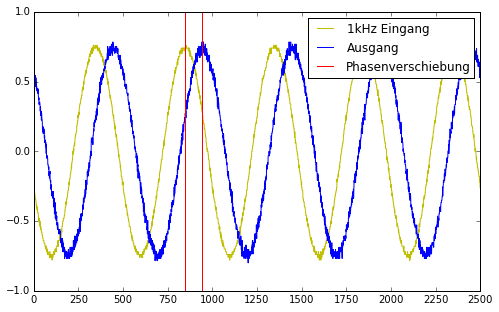
\includegraphics[width=80mm]{ein-ausgang.png}
\caption{Eingangsignal Lautsprecher und Ausgangssignal Mikrofon}
\label{img:EingangAusgang}
\end{figure}

\begin{figure}[H]
\centering
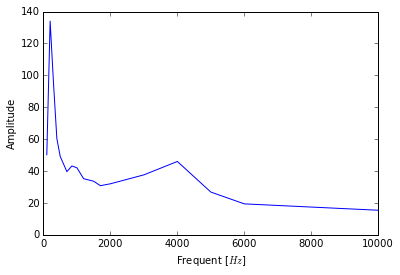
\includegraphics[width=80mm]{amplitude_gross.png}
\caption{Amplitude Lautsprecher gross}
\label{img:AmplitudeLGross}
\end{figure}

\begin{figure}[H]
\centering
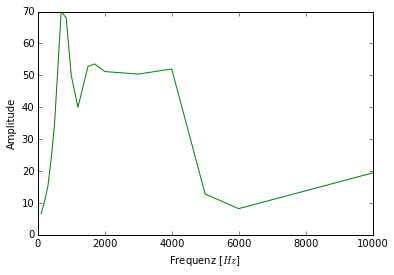
\includegraphics[width=80mm]{amplitude_klein.png}
\caption{Amplitude Lautsprecher klein}
\label{img:AmplitudeLklein}
\end{figure}

\begin{figure}[H]
\centering
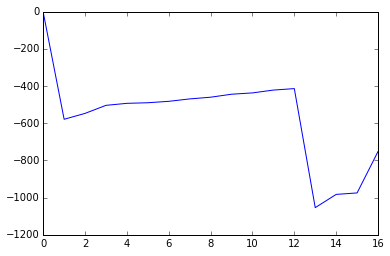
\includegraphics[width=80mm]{phase_gross.png}
\caption{Phase Lautsprecher Gross}
\label{img:phase_gross}
\end{figure}

\begin{figure}[H]
\centering
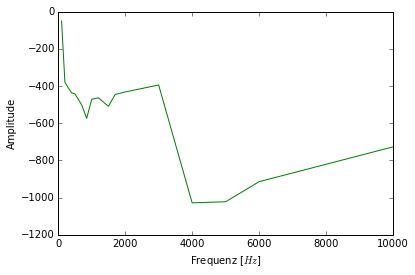
\includegraphics[width=80mm]{phase_klein.png}
\caption{Phase Lautsprecher klein}
\label{img:PhaseKlein}
\end{figure}

\begin{figure}[H]
\centering
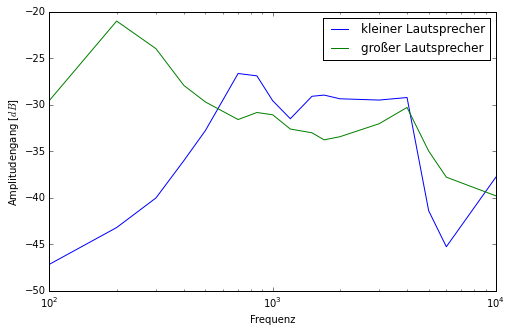
\includegraphics[width=120mm]{amplitudengang.png}
\caption{Bode-Diagramm Amplitudengang}
\label{img:BodeAmplitude}
\end{figure}

\begin{figure}[H]
\centering
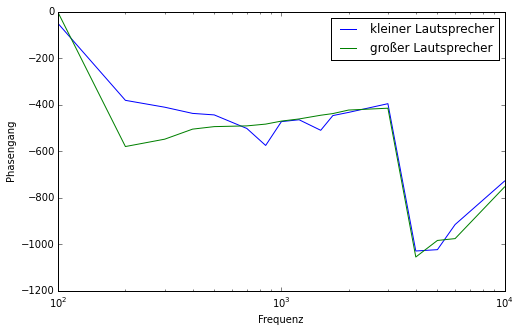
\includegraphics[width=120mm]{Phasengang.png}
\caption{Bode-Diagramm Phasengang}
\label{img:PhasenGang Bode-Diagramm}
\end{figure}


\section{Auswertung und Interpretation}
\label{chap:AUSWERTUNGUNDINTERPRETATION}
In Abbildung \ref{img:EingangAusgang} ist das Signal vom Sinusgenerator in Gelb und das Aufgenommene Signal in Blau zu sehen. Die Vertikalen Linien zeigen die Phasenverschiebung der beiden Signale an. Auf diesem Bild scheinen sich die Amplituden nicht zu unterscheiden. Dies hängt aber lediglich von der Skalierung der einzelnen Kurven im Oszilloskop ab. Die eigentlichen Amplituden sind den Tabellen \ref{tab:MLg} und \ref{tab:MLk} zu entnehmen. Bei der Abbildung handelt es sich nur um eine Beispielhaftes Signal, welche nachträglich zum Versuch aufgenommen wurde. Leider ist auf dieser Abbildung kein Unterschied der Amplituden zu sehen.

Um den Frequenzgang des linearen Systems Lautsprecher zu bestimmen interessiert der jeweilige Amplitudengang, sowie der Phasengang. Da der Amplitudengang nicht in Abhängikeit der Eingangsspannung von 1.5 V bestimmt werden soll, wird für das Bode-Diagramm das Verhältnis bestimmt. In Abbildung \ref{img:AmplitudeLGross} bzw. \ref{img:AmplitudeLklein} sind trotzdem nochmal die Amplitudenverläufe für die entsprechenden Frequenzen zu sehen. Die Messung der Phasenverschiebungen sind ebenfalls in zwei Diagrammen aufgetragen, so dass man für jede gemessene Frequenz sehen kann, wie sich die Phasenverschiebung verhält. Das Verhalten der Lautsprecher im Bezug auf die Amplitude und die Phase soll im Kontext mit den Bode-Diagrammen diskutiert werden.

Im Bode-Diagramm für die Amplituden wird die Frequenz auf der X-Achse zur Basis 10 logarithmiert. Der Betrag des Wertebereiches wird ebenfalls logarithmiert und mit Zwanzig multipliziert. Damit erhält man einen Amplitudenfaktor in DeziBel. Es handelt sich also nicht um eine bestimmte Amplitude zu einer bestimmten Frequenz in diesem Schaubild, sondern viel mehr um einen Faktor, der mit dem Eingangssignal des Systems multipliziert wird. Dieses Signal erhält je nach Frequenz eine andere Anpassung der Amplitude durch diesen Faktor. Dieser Faktor ist also in Abhängigkeit von der Frequenz der Amplitudengang.
In Schaubild \ref{img:BodeAmplitude} ist der Amplitudengang des großen, sowie auch des kleinen Lautsprechers zu sehen.
Es kann also nun das Verhalten beider Lautsprecher miteinander verglichen werden. In beiden Fällen findet keine Verstärkung des Signals statt. Dies ist auch nicht weiter verwunderlich, da es sich bei Lautsprechern um passive Elemente handelt. Daher würde jedes andere Verhalten den Hauptsätzen der Thermodynamik widersprechen.
Der große Lautsprecher hat seine geringste Dämpfung im gemessenen Bereich von 100 bis $\approx 500$ Hertz. In diesem Bereich findet sich der Breakevenpoint von großem und kleinem Lautsprecher wieder. Im Bereich von $\approx 500$ bis $\approx 1300$ Hertz hat der kleine Lautsprecher den höheren Wirkungsgrad. In diesem Diagramm wird ersichtlich, das der Große Lautsprecher für die tieferen Frequenzen den höheren Wirkungsgrad hat und der kleine in den höheren.


